\section{Pregled cjevovoda za detekciju}
\label{sec:pregled-cjevovoda}

Cjevovod za detekciju grane obrađuje isključivo slikovnu ravninu i ne sadrži ugrađenu pretpostavku o fizičkoj orijentaciji kamere u prostoru. Cjevovod za detekciju grane nije zaseban proces koji radi usporedno s praćenjem, nego je ugniježđen unutar iste petlje: dok konačna točka nije zaključana, svaka iteracija ove petlje poziva cjevovod za detekciju za sljedeću sličicu i iz njega čita trenutno stanje. Tek nakon zaključavanja petlja prestaje pozivati cjevovod za detekciju i prelazi na izravno čitanje sirovih sličica s kamere, a praćenje preuzima KLT algoritam opisan u nastavku (Odjeljak~\ref{subsec:klt}). Izlaz cjevovoda prema upravljačkom sloju ostaje par vrijednosti procijenjenog položaja točke prijanjanja u slikovnoj ravnini (\texttt{point\_x}, \texttt{point\_y}).

\section{Skup podataka i treniranje modela}
\label{sec:treniranje-modela}

Detekcija grana za primjene na UAV-u dosad je istraživana u nekoliko smjerova. Silva i sur.~\cite{SILVA2022102759} predložili su metodu detekcije linija temeljenu na konvolucijskoj neuronskoj mreži za prepoznavanje grana stabla iz digitalnih fotografija, koristeći Houghovu transformaciju za procjenu orijentacije grane i točke prihvata. Lin i sur.~\cite{lin2025performanceevaluationdeeplearning} usporedili su nekoliko modela dubokog učenja za segmentaciju u autonomnim šumarskim sustavima, dajući usporedbu performansi modela u stvarnim uvjetima. Oba rada usredotočena su isključivo na percepcijsku stranu problema, bez obrade cjelokupnog cjevovoda od detekcije do upravljanja, za razliku od njih, model korišten u ovom radu dio je cjelovitog cjevovoda opisanog u nastavku ovog poglavlja.

\subsection{Skup podataka i označavanje}
Izbor modela za segmentaciju instanci umjesto obične detekcije izravna je posljedica zahtjeva za pikselnom preciznošću točke prijanjanja. Okvir za detekciju (\emph{bounding box}) daje samo grubu procjenu položaja i veličine grane, dok manevar prijanjanja zahtijeva mnogo precizniju procjenu: pogreška od svega nekoliko centimetara u stvarnom prostoru dovoljna je da hvataljka fizički promaši granu. Maska na razini piksela, za razliku od okvira, omogućuje izdvajanje znatno preciznije točke unutar same grane, što je motivacija za korištenje segmentacijskog, a ne isključivo detekcijskog modela.

Skup podataka za treniranje preuzet je s Roboflowa~\cite{branch-dataset_dataset} i sadrži 1365 slika za treniranje, 390 za validaciju i 203 za testiranje, sve iz jedne klase (grana), izvorno označene okvirima za detekciju objekata. Budući da je za ovaj rad potrebna preciznost na razini piksela, a ne samo okvir, maske za segmentaciju automatski su generirane modelom SAM3 (Segment Anything Model 3) tvrtke Meta~\cite{carion2026sam3segmentconcepts}, na temelju tekstualnog upita "tree branch", čime se izbjeglo ručno označavanje gotovo 2000 slika. Puna segmentacija cijele scene izravnim pokretanjem SAM3 na ulazne okvire razmatrana je, ali odbačena kao računalno prezahtjevna za izvođenje na Raspberry Pi računalu.

\subsection{Treniranje i usporedba modela}
Treniranje je provedeno korištenjem Ultralytics biblioteke, koja objedinjuje sučelje za treniranje, validaciju i izvoz YOLO modela. Segmentacijski model YOLOv8m-seg treniran je 300 epoha, uz praćenje napretka na platformi Weights \& Biases. Usporedba je provedena i s modelom YOLOv26-seg treniranim pod istim uvjetima: YOLOv8m-seg dosljedno je nadmašio YOLOv26-seg po gotovo svim mjerama (npr. mAP50-95 na razini okvira približno 0,63 naspram 0,58), a uz to je i jedina opcija podržana za izvoz u format koji AI Hat+ prihvaća, budući da akcelerator podržava samo YOLO modele do verzije 8. YOLOv8m-seg stoga je odabran po oba kriterija.

Gubitci na skupu za treniranje i validaciju padaju i konvergiraju kroz svih 300 epoha, što ukazuje da model ne prenaučava (\emph{overfitting}) na skup za treniranje. Većina učenja odvija se unutar prvih 150 epoha, nakon čega mjere počinju stagnirati. mAP50 na razini okvira dosegnuo je približno 0,75 do kraja treniranja, što je razuman rezultat s obzirom na težinu zadatka: razlikovanje tanke, granate grane od pozadine sličnog izgleda (druge grane, sjene, tekstura kore) u prirodnom okruženju.

\begin{figure}[htb]
\centering
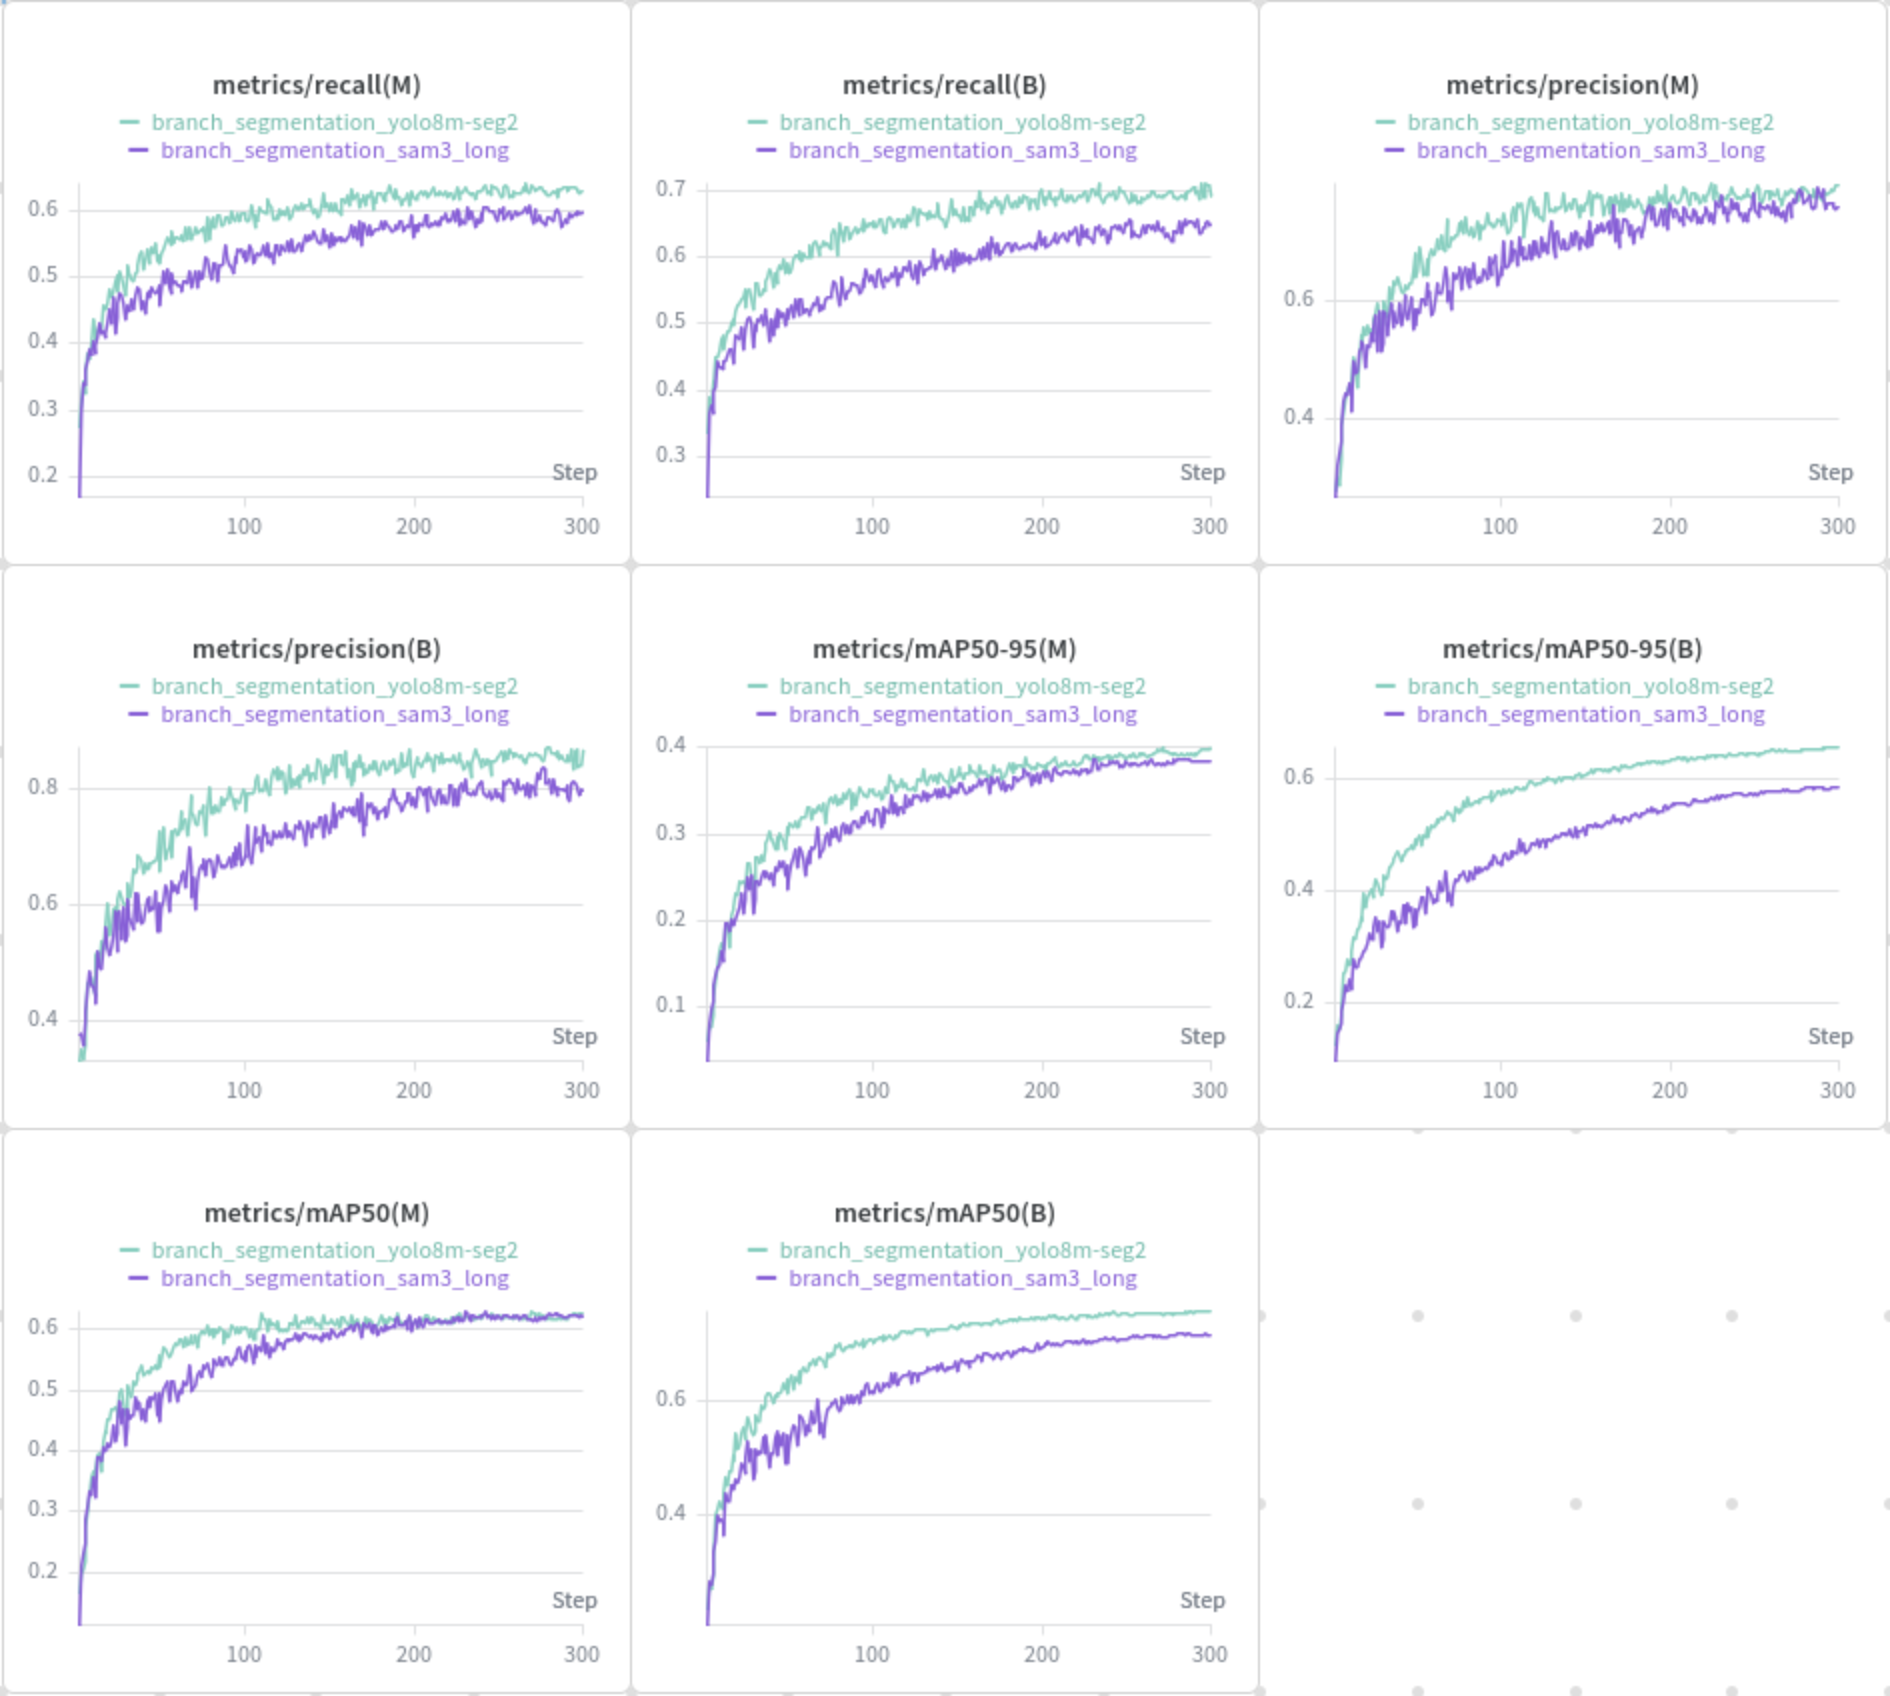
\includegraphics[width=1.0\textwidth]{images/metrics_compare.png}
\caption{Usporedba mjera treniranja modela YOLOv8m-seg i YOLOv26-seg kroz 300 epoha (odziv, preciznost i mAP na razini maske (M) i okvira (B)).}
\label{fig:metrics_compare}
\end{figure}

\subsection{Kvantizacija i izvođenje na rubnom uređaju}
\label{subsec:kvantizacija}
Nakon treniranja, težine modela izvezene su iz PyTorch (\texttt{.pt}) formata u ONNX, standardizirani format koji omogućuje prijenos modela između različitih okvira i sklopovlja. ONNX model potom je kompiliran u Hailo izvršni format (\texttt{.hef}) korištenjem Hailo AI Software Suite alata, koji Hailo distribuira kao Docker sliku sa svim potrebnim alatima. Nakon kvantizacije, brzina izvođenja modela na AI Hat+ akceleratoru ovisi o vrsti detekcije i broju grana prisutnih u kadru: unatoč tome što kamera isporučuje 30 sličica u sekundi, obrada na Raspberry Pi 5 pri stvarnoj detekciji grana usporava izlaznu frekvenciju cjevovoda na oko 4,6 Hz. Ovo usko grlo izravan je razlog uvođenja KLT praćenja nakon zaključavanja točke prijanjanja (vidi Odjeljak~\ref{subsec:klt}), koje zaobilazi ponovljeno pokretanje modela detekcije za svaku sličicu.

% TODO: napomenuti u Raspravi da skup podataka trenutno ne sadrzi fotografije grana
% snimljene iz perspektive kamere okrenute prema gore (nebo kao pozadina), sto moze
% utjecati na tocnost detekcije u novoj konfiguraciji

\section{Praćenje točke prijanjanja (KLT)}
\label{subsec:klt}

\begin{figure}[htb]
\centering
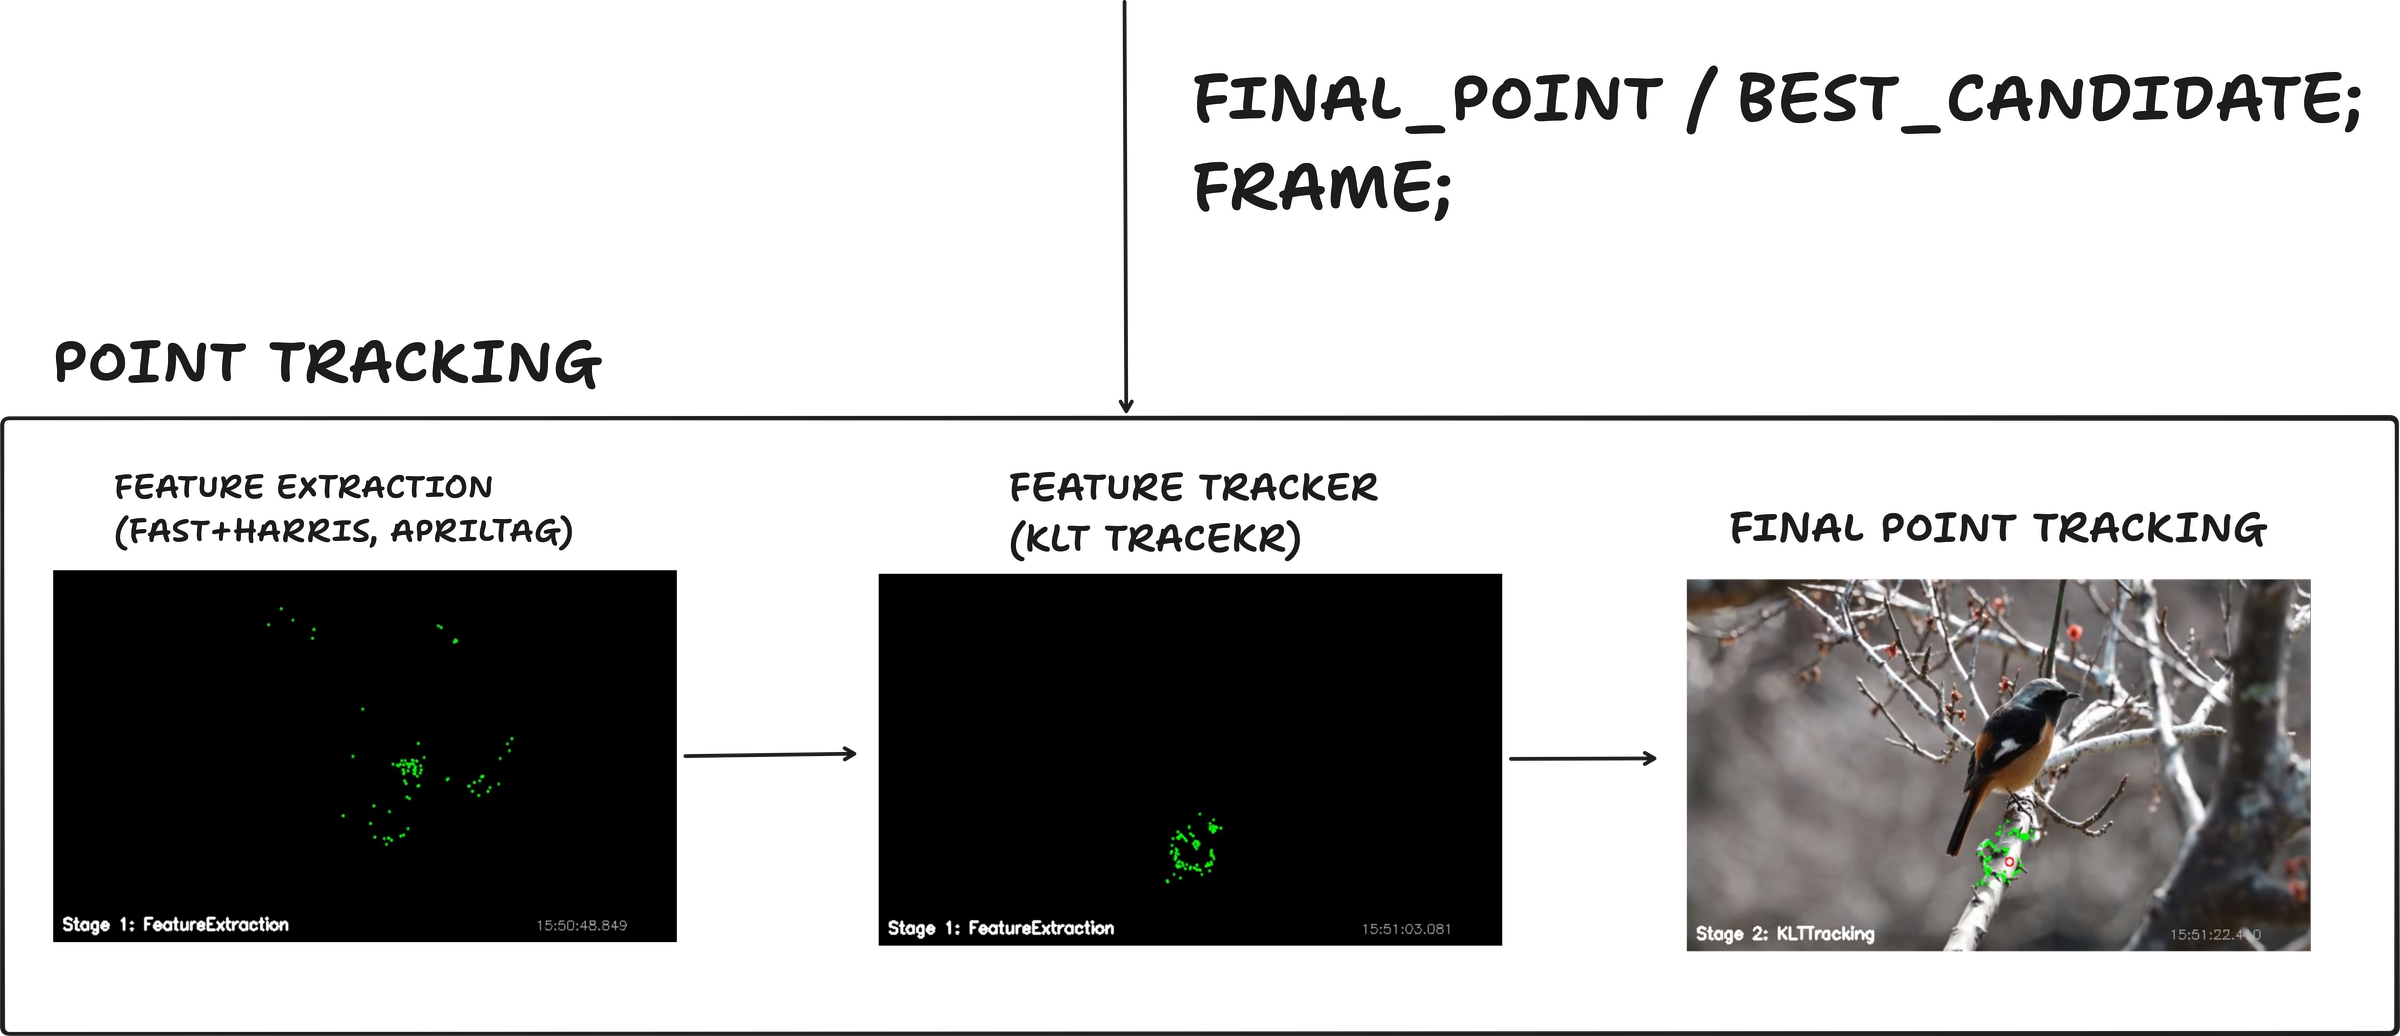
\includegraphics[width=1.0\textwidth]{images/point_tracking_overview.png}
\caption{Integracija cjevovoda za detekciju s praćenjem točke prijanjanja: izdvajanje značajki, KLT praćenje i procjena položaja konačne točke.}
\label{fig:ibvs_overview}
\end{figure}

Nastavak oslanjanja na model segmentacije nakon zaključavanja točke bio bi neopravdano skup: kako je pokazano u Odjeljku~\ref{subsec:kvantizacija}, izlazna frekvencija modela detekcije pri stvarnoj detekciji grana pada na oko 4,6 Hz, dok upravljački sloj zahtijeva znatno češće ažuriranje cilja. Umjesto ponovnog pokretanja modela, praćenje se stoga oslanja isključivo na optički tok, koji je računalno jeftiniji i ne ovisi o ponovljenom uspješnom prepoznavanju grane u svakoj sličici. Ovo praćenje izvodi se u potpunosti na strani Raspberry Pi OS-a, kao dio istog procesa koji izvodi cjevovod za detekciju, za razliku od upravljačke IBVS petlje opisane u poglavlju~\ref{ch:upravljanje}, koja se izvodi zasebno, na Docker strani sustava.

Nakon zaključavanja konačne točke, KLT tracker izdvaja FAST i Harris kutne značajke iz referentne slike u lokalnoj okolini točke prijanjanja te pohranjuje pomak svake značajke u odnosu na tu točku.

U svakoj sljedećoj slici značajke se prate KLT (\emph{Kanade--Lucas--Tomasi}) algoritmom optičkog toka na piramidalnoj reprezentaciji slike, a položaj točke prijanjanja procjenjuje se kao trenutno središte (centroid) uspješno praćenih značajki. Time se izbjegava ponovno pokretanje modela detekcije za svaku sliku, čime se smanjuje računalno opterećenje i omogućuje praćenje znatno većom frekvencijom nego što bi to dopuštalo izvođenje modela segmentacije nad svakim okvirom.

\begin{figure}[htb]
\centering
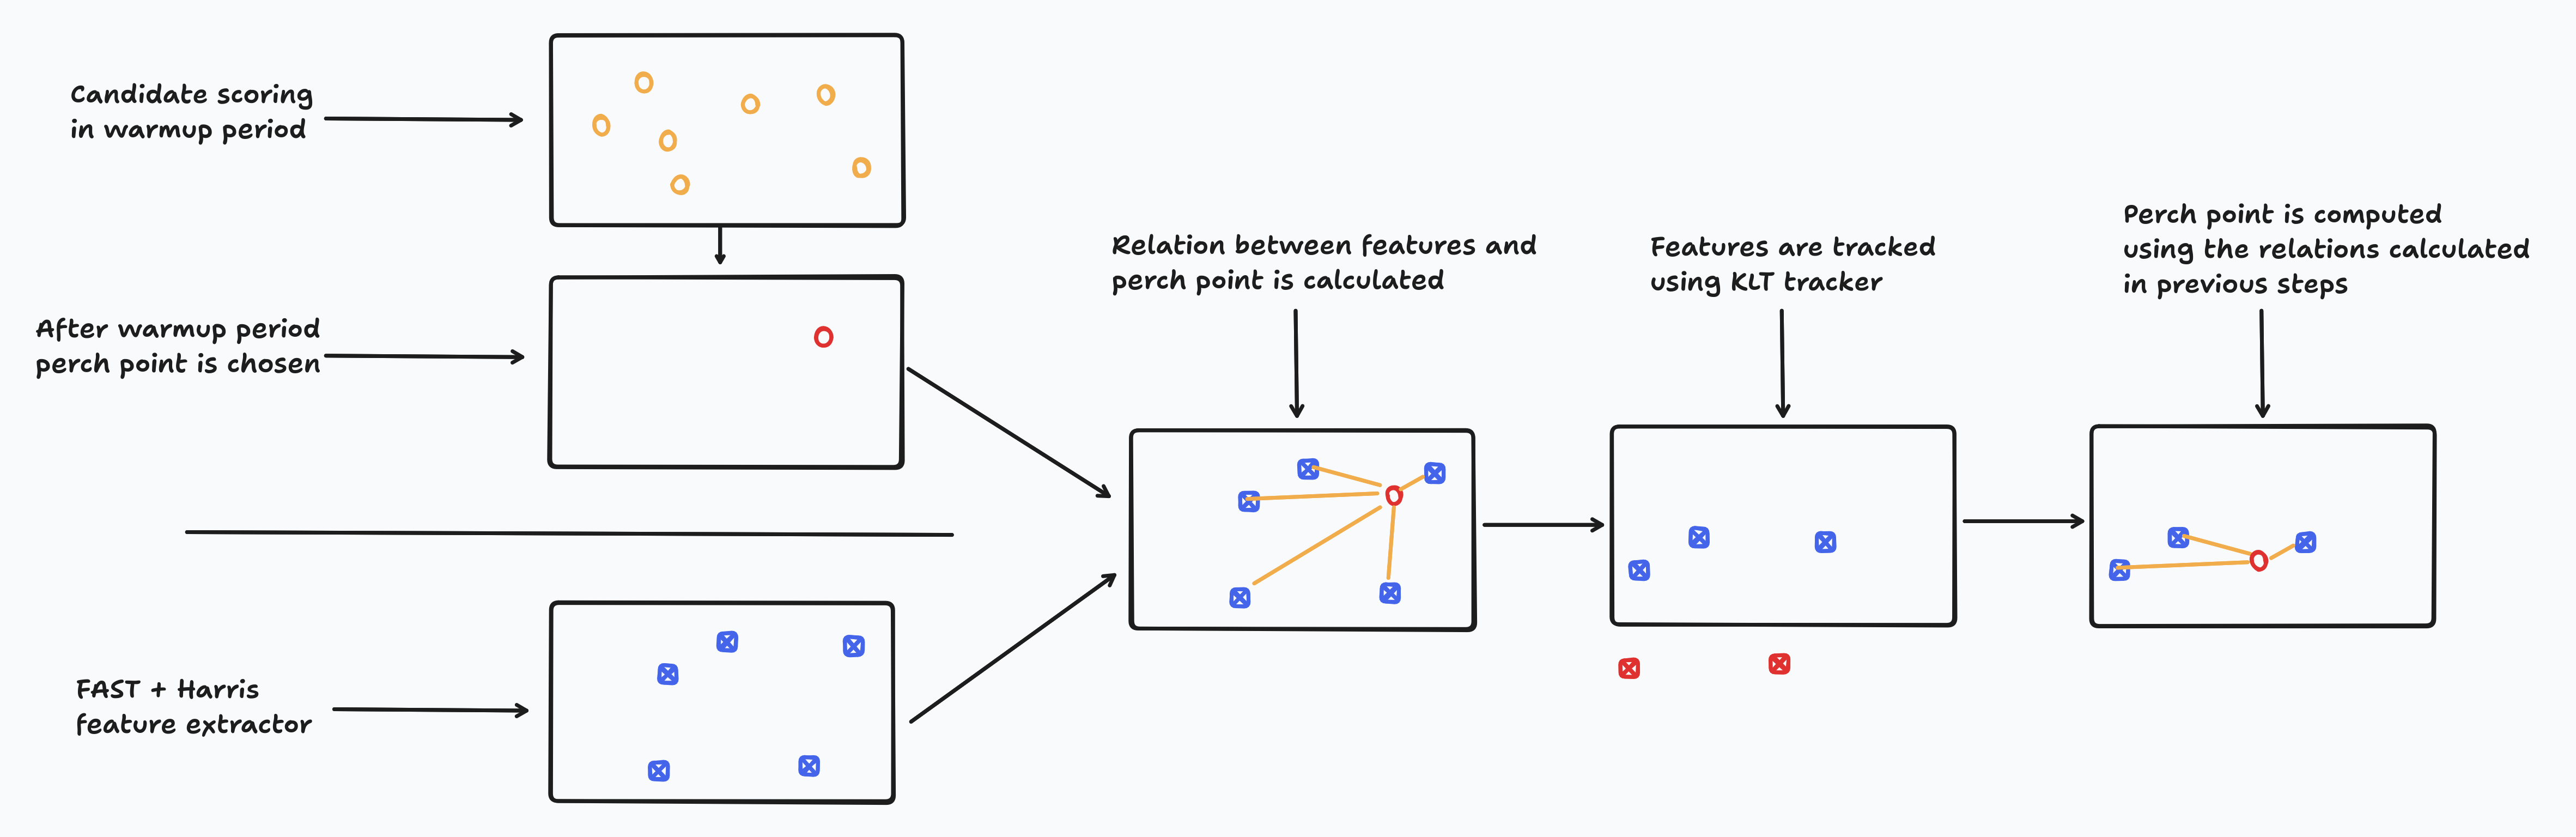
\includegraphics[width=1.0\textwidth]{images/final_point_tracking.png}
\caption{Postupak procjene položaja točke prijanjanja: odnos između izdvojenih značajki i zaključane točke fiksira se u trenutku zaključavanja, a nakon svakog koraka KLT praćenja taj se fiksni odnos primjenjuje na nove položaje značajki kako bi se odredio procijenjeni položaj točke. Testni video~\cite{pixabay_bird_video}.}
\label{fig:final_point_tracking}
\end{figure}

Praćenje uključuje provjeru dosljednosti unaprijed-unatrag (\emph{forward-backward}): svaka procijenjena nova pozicija značajke prati se i unatrag u prethodnu sliku, a značajke čiji povratni položaj odstupa od izvornog odbacuju se kao nepouzdane. Ako broj preživjelih značajki padne ispod praga, značajke se ponovno izdvajaju oko predviđenog položaja središta (na temelju posljednje zabilježene brzine pomaka), umjesto oko posljednjeg poznatog položaja, čime se ponovno izdvajanje bolje prilagođava kretanju cilja. Dodatno, ako se središte praćenih značajki ne pomiče kroz veći broj uzastopnih slika, praćenje se proglašava nepouzdanim i signalizira se gubitak cilja, čime se sprječava da sustav neprimjetno prati nepomičnu pozadinu umjesto stvarnog cilja.

Pogreška u odnosu na središte slike ovdje se ne računa: taj izračun, kao i preslikavanje u naredbe letjelici, u potpunosti je izmješten u upravljačku IBVS petlju opisanu u poglavlju~\ref{ch:upravljanje}, koja se izvodi zasebno, na Docker strani.
